% TODO add tech / software table?
\section{Materials and methods}

\subsection{Study design}

% Brief overview
At a general level the study constituted two main parts:
the development of the map presentation and
the survey to find out how
people use and understand the presentation.
While the primary goal of the development process was
to produce the map presentation and enable the survey,
the development process in and of itself was crucial to the study as well.
Its purpose was to be the framework that
allows me to test and answer my research questions
about the more technology-centric aspects of
making of an interactive map.

So, a large part of this study was
in essence a software development project,
and the parts that were not, were still reliant on
the software development project succeeding.
This kind of setting,
combined with the author's limited experience with the relevant technologies,
inherently introduced a high level of risk and uncertainty to the study.
To minimize these factors,
I heavily utilized modern software development methodologies
\parencite{saq2020, bec2001, sha2017} in planning the development process
and designing the study.
Based on these,
I formatted the following points of focus
to guide the development process:
\begin{itemize}
	\item Plan minimally and adapt the plan constantly.
	\item Prioritize a working state of the entire system over details in single components.
	\item Adapt to technical constraints at the start, not at the end.
\end{itemize}

By adhering to these principles I could at an early stage see whether the system --
and, by extension, the entire study -- is realistic.
It also made it possible for me to avoid wasted effort and, most importantly,
make sure I am developing a system that is valuable to the entire study.
Iteratively improving the system as a functional whole
allowed me to consider the map interface
from the perspective of the map user as early as possible,
better integrating the survey into the study.
This is important as the map presentation is simultaneously an output of the development process
and an input to the design of the survey.

For an overview of the study design see figure \ref{fig:study design}.
% This allowed me to improve the relevancy of my research. TODO Discussion?
% I say this not only in the context of gaining valuable results to my research questions --
% I want to emphasize that to even know what research questions to ask is impossible with a linear approach.

% While the development process and the survey were linked to each other,
% they each had their separate goals and outputs too.
% In addition to producing the map presentation,
% the development process had to enable testing and answering my research questions
% about the making of an interactive map.
% This placed increased
% The goal of the survey is to gain insight on
% how the interactive map works as a representation of the mapped phenomenon.
% With the survey I collect data on map usage,
% which I in turn analyse to answer my research questions related to the map usage.

\begin{figure}[H]
	\centering
	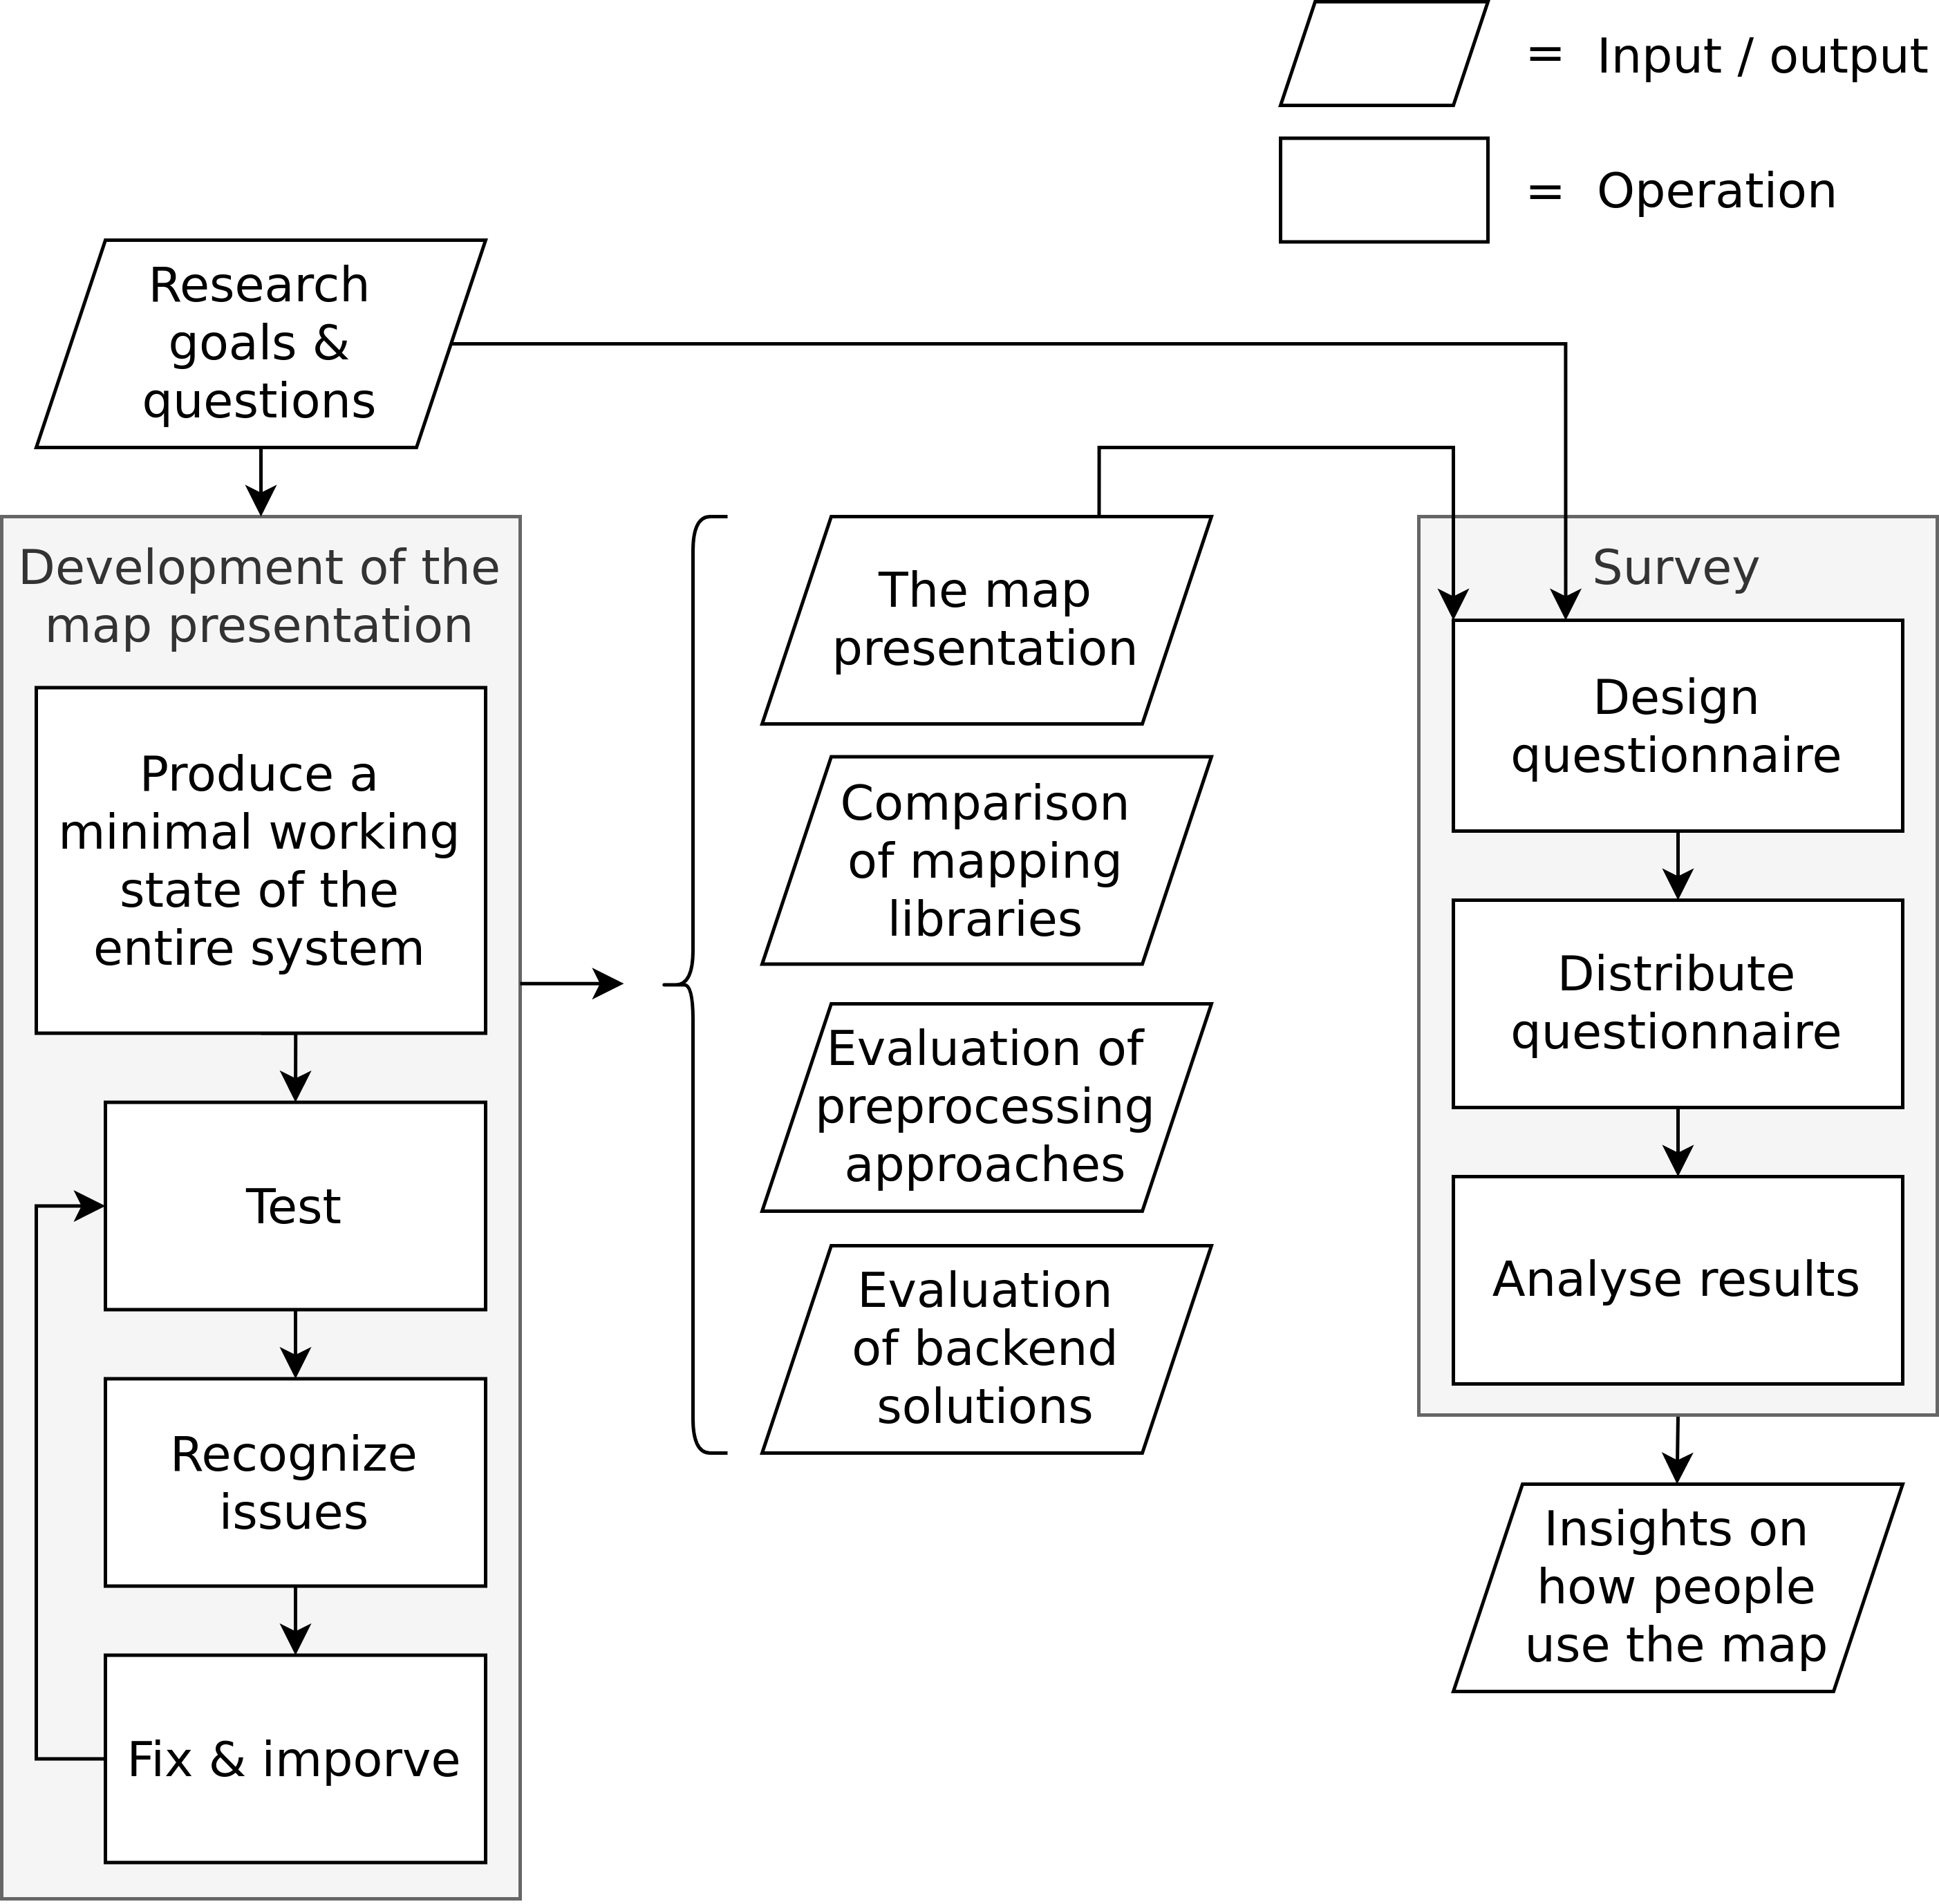
\includegraphics[width=0.8\textwidth]{visual/figures/diagrams/study_design.png}
	\caption{An overview of the study design}
	\label{fig:study design}
\end{figure}


\subsection{Data -- Helsinki region Travel Time Matrix}

The \acrlong{ttm} (\acrshort{ttm}) \parencite{fin2023}
is a dataset containing information of travel times and distances
in the Helsinki region in southern Finland.
This dataset was crucial to developing the map application,
as it was the sole source of the travel times shown on the map.
The dataset and the set of methods with which it is produced are open-source.

% Describe ttm in general: ykr, origin dest pairs etc (more surface level stuff common to all matrices)
A significant component of the \acrshort{ttm} is the \acrlong{ykr} (\acrshort{ykr})
statistical grid made by the Finnish Environmental Institute.
The grid has a spatial resolution of 250x250m, and it covers the entire Finland.
Most importantly, however, the part of the \acrshort{ykr} grid that overlaps with
the Helsinki region provides the spatial component for
the travel times stored in the \acrshort{ttm}.
The spatial extent of the dataset is shown in \ref{fig:ttm extent}.

\begin{figure}[H]
	\centering
	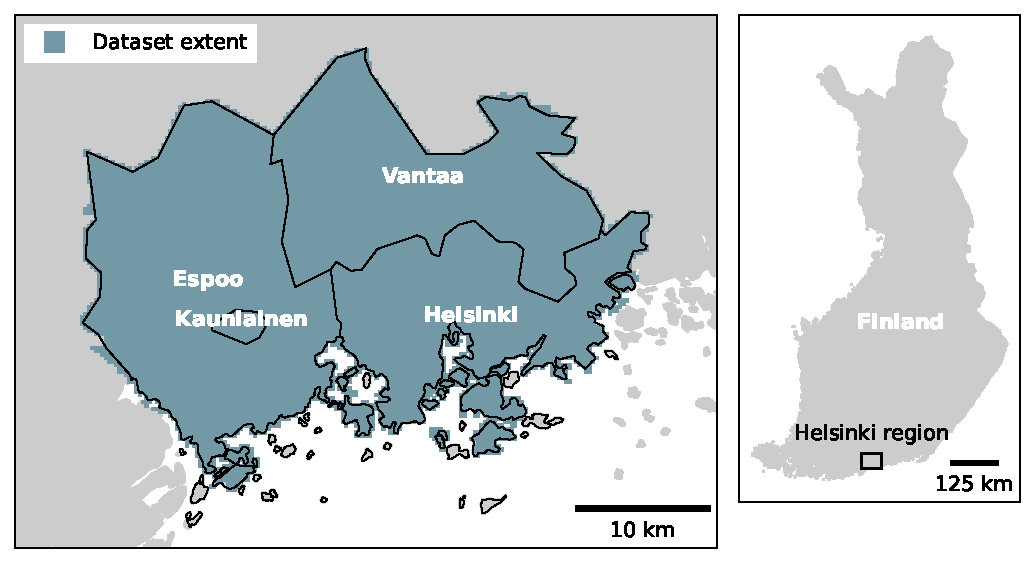
\includegraphics[width=0.9\textwidth]{visual/figures/ttm/ttm_extent.pdf}
	\caption{The location and extent of the TTM}
	\label{fig:ttm extent}
\end{figure}

The \acrshort{ttm} stores the travel times and distances
from every \acrshort{ykr} grid cell to every other  \acrshort{ykr} grid cell
within the Helsinki region.
The Helsinki region fits 13231 \acrshort{ykr} grid cells,
which means that the complete \acrshort{ttm} contains travel times and distances for
over 175 million routes.

All the routes are calculated for multiple different travel modes.
The primary travel modes are walking, cycling, public transportation and private car,
and, when applicable, each mode has variations based on
time of day and / or walking or cycling speed.
Time of day is especially relevant to motorized transport
in the form of the rush hour, for example,
while walking speed affects any travel mode
where a significant portion of the trip is covered on foot.
% Modelling the travel times accounts for walking,
% transfer times based on public transit schedules,
% and the actual geometries of the routes.

% TODO talk briefly about methodology, open source

% Describe the particular matrix (2023), methodology etc
\acrshort{ttm}s have been calculated for multiple years.
Differences between these datasets exist in the applied methodologies and thus the content
\parencite{ten2020}.
Also, the underlying city structure is by no means static over the years
which further introduces differences.
The map presentation I develop here is based on the 2023 version of the \acrshort{ttm},
the newest one at the time of writing.
See table \ref{tab:ttm description} for an overview of the dataset,
and table \ref{tab:ttm table structure} for all the travel modes in the dataset.

\begin{table}[H]
	\caption{Descriptive values of the \acrshort{ttm}}
	\label{tab:ttm description}
	\centering
	\begin{tabular}{ | L{0.4\textwidth} | L{0.5\textwidth} | }
		\hline
		Spatial resolution
		& 250 x 250 m
		\\
		\hline
		Number of grid cells
		& 13231
		\\
		\hline
		Number of origin-destination pairs
		& 175 059 361
		\\
		\hline
		Travel modes
		& \tabitem walking \\
		& \tabitem cycling \\
		& \tabitem public transportation \\
		& \tabitem private car \\
		\hline
		Travel mode variations (if applicable)
		& \tabitem Time of day (rush hour, midday, night) \\
		& \tabitem Walking speed (average, slow) \\
		& \tabitem Cycling speed (average, fast, slow) \\
		\hline
	\end{tabular}
\end{table}


\begin{table}[H]
	\caption{The table structure of \acrshort{ttm} data}
	\label{tab:ttm table structure}
	\centering
	\begin{tabular}{ | L{0.15\textwidth} | L{0.75\textwidth} | }
		\hline
		\textbf{Column name}
		& \textbf{Description}
		\\
		\hline
		\hline
		from\_id
		& ID number of the origin grid cell
		\\
		\hline
		to\_id
		& ID number of the destination grid cell
		\\
		\hline
		walk\_avg
		& Travel time in minutes from origin to destination by walking at an average speed
		\\
		\hline
		walk\_slo
		& Travel time in minutes from origin to destination by walking slowly
		\\
		\hline
		bike\_avg
		& Travel time in minutes from origin to destination by cycling at an average speed; incl. extra time (1 min) to unlock and lock bicycle
		\\
		\hline
		bike\_fst
		& Travel time in minutes from origin to destination by cycling fast; incl. extra time (1 min) to unlock and lock bicycle
		\\
		\hline
		bike\_slo
		& Travel time in minutes from origin to destination by cycling slowly; incl. extra time (1 min) to unlock and lock bicycle
		\\
		\hline
		pt\_r\_avg
		& Travel time in minutes from origin to destination by public transportation in rush hour traffic, walking at an average speed
		\\
		\hline
		pt\_r\_slo
		& Travel time in minutes from origin to destination by public transportation in rush hour traffic, walking at a slower speed
		\\
		\hline
		pt\_m\_avg
		& Travel time in minutes from origin to destination by public transportation in midday traffic, walking at an average speed
		\\
		\hline
		pt\_m\_slo
		& Travel time in minutes from origin to destination by public transportation in midday traffic, walking at a slower speed
		\\
		\hline
		pt\_n\_avg
		& Travel time in minutes from origin to destination by public transportation in nighttime traffic, walking at an average speed
		\\
		\hline
		pt\_n\_slo
		& Travel time in minutes from origin to destination by public transportation in nighttime traffic, walking at a lower speed
		\\
		\hline
		car\_r
		& Travel time in minutes from origin to destination by private car in rush hour traffic
		\\
		\hline
		car\_m
		& Travel time in minutes from origin to destination by private car in midday traffic
		\\
		\hline
		car\_n
		& Travel time in minutes from origin to destination by private car in nighttime traffic
		\\
		\hline
		walk\_d
		& Distance from origin to destination, in metres, on foot
		\\
		\hline
	\end{tabular}
\end{table}




\subsection{Implementation of the map presentation}

\subsubsection{Software requirements}
% The requirements of the system are an essential aspect to consider,
% since they
% For example, the sheer scale and detail of the dataset being visualized
% means that instantaneous interaction with the map is not realistic
% if no detail of the mapped data is to be sacrificed.
% These kinds of tradeoffs are important to recognize,
% because only through them is it possible to specify what
% requirements should, or even could, be placed on the map application.

% TODO copypasta

% Roughly what kind of a map? Why?
% Based on the background study,  % TODO
Software requirements are functionalities and properties
that a given system should have \parencite{chu2009}.
They are an essential aspect to consider in all software development
as they dictate much of how any implementation is carried out \parencite{saq2020}.
Software requirements are often divided into
functional and nonfunctional requirements.
Functional requirements define the user-facing features of the system
while nonfunctional requirements describe the properties of a system
\parencite{chu2009}.
Nonfunctional requirements can be further divided into
quality attributes and constraints.
Quality attributes describe \textit{how} the software should be,
while constraints mean technical limitations \parencite{chu2009}.

I based the requirements of this particular system on the goals of the study,
considering the interactive map presentation.
The starting point for specifying these requirements
was my decision to prioritize real-time interaction over minute detail in the map.
The goal of the map interface was to act as a dynamic overview to the entire \acrshort{ttm}.
As mentioned above, the spatial dimension of the \acrshort{ttm} is large,
so, if all of it is to be explored,
selecting different locations must be effortless and instantaneous.
The other dimension, travel mode, is much smaller,
but it should also be interactively selectable.
These two goals, while still quite vague,
immediately placed a number of requirements on the system.
From the perspective of the user,
there must be functionalities for interacting with the map to
select different locations, preferably very rapidly,
and different travel modes.
A significant quality attribute to consider is that the system should
support instantaneous real-time interactivity.
Also at the very start I made the decision to target the web as the platform.
This constraint was the starting point for considering the technologies
for carrying out the implementation.
% To achieve this, the latency between user input and
% its visible results must be minimized.

In accordance with the guideline of continuous adaptation
\parencite{bec2001} I specified the software requirements loosely at first,
further focusing them as the system took shape.
To communicate the development process in an orderly manner,
and to motivate the design decisions I've made, I present
the requirements of the final system here.
Still, I should emphasize that the reality is not this linear.

The functional requirements (table \ref{tab:functional requirements})
comprise two modes of interaction for selecting locations:
clicking the map with a pointing device to produce a static map of the clicked location,
and continuously changing the location by moving the mouse over the map
(referred to as hovering).
I also specify that interface capabilities for selecting travel modes
and changing the mode of location selection should be present.
For the quality attributes of the system (table \ref{tab:quality attributes})
performance is an essential consideration,
both in the sense of software performance
and the responsiveness of the application as perceived by the user.
This must be considered in both the front- and backend of the system.
Other important aspects are that the system can be maintained and deployed,
and that it can meet different real-world usage loads --
if these attributes were lacking,
the work I've carried out would have little real value,
as it would be left available only to me.
As mentioned earlier,
the application is constrained to running in a web browser (table \ref{tab:constraints}).
Also -- as a general best-practice, as well as a constraint
necessitated by the available deployment environment --  % ref csc?
the implementation must be completely containerized (table \ref{tab:constraints}).

\begin{table}[H]
	\caption{The functional requirements of the map application}
	\label{tab:functional requirements}
	\centering
	\begin{tabular}{ | L{0.3\textwidth} | L{0.6\textwidth} | }
		\hline
		Requirement
		& Description
		\\
		\hline
		\hline
		Location selection by clicking
		& The user can click on a location and produce an accessibility map of that location.
		\\
		\hline
		Location selection by hovering
		& The user can hover their mouse over the map,
		and the map shows the accessibility of the location that is under the cursor,
		updating constantly as the cursor moves.
		\\
		\hline
		Toggling between modes of location selection
		& The user can toggle their mode of interaction by clicking:
		Clicking while hovering locks the map, clicking while the map is locked resumes hovering.
		\\
		\hline
		Interactive selection of travel mode
		& The user can choose the travel mode for which the travel times shown on the map are calculated.
		\\
		\hline
	\end{tabular}
\end{table}

\begin{table}[H]
	\caption{
		The nonfunctional requirements of the map application specify
		its desired qualities (\ref{tab:quality attributes}) and
		the constraints it must adhere to (\ref{tab:constraints}).
	}
	\label{tab:nonfunctional requirements}
	\begin{subtable}[h]{\textwidth}
		\caption{}
		\label{tab:quality attributes}
		\centering
		\begin{tabular}{ | L{0.2\textwidth} | L{0.7\textwidth} | }
			\hline
			\textbf{Category}
			& \textbf{Requirements}
			\\
			\hline
			\hline
			Performance
			& \tabitem Data serving speed allows for real-time interaction. \\
			& \tabitem Map rendering speed allows for real-time interaction. \\
			\hline
			Maintainability
			& \tabitem All components are as independent as possible. \\
			& \tabitem The codebase is versioned and documented. \\
			& \tabitem Deploying the application is reproducible. \\
			\hline
			Usability
			& \tabitem Visual feedback from user interaction is instantaneous. \\
			\hline
			Scalability
			& \tabitem The application is scalable to meet different usage loads. \\
			& \tabitem Different application components can be scaled independently. \\
			\hline
		\end{tabular}
	\end{subtable}
	\newline
	\newline  % https://tex.stackexchange.com/questions/38893/cant-generate-vertical-space-between-tables
	\newline
	\begin{subtable}[h]{\textwidth}
		\caption{}
		\label{tab:constraints}
		\centering
		\begin{tabular}{ | L{0.2\textwidth} | L{0.7\textwidth} | }
			\hline
			\textbf{Type of constraint}
			& \textbf{Description}
			\\
			\hline
			\hline
			Client-side platform
			& The frontend of the map application runs in a web browser.
			\\
			\hline
			Deployment environment
			& The front and backend are deployed in containers
			utilizing the OpenShift container platform.
			\\
			\hline
		\end{tabular}
	\end{subtable}
\end{table}


\subsubsection{Data preprocessing}
Considering the requirements, the \acrshort{ttm}
To make the \acrshort{ttm} mappable, it must be at some point of the
To enable real-time interactivity with the map the travel time

% The need for preprocessing
% - what would raw data be like?
% - why as much as possible should be precalculated
% && the requirements preprocessing must satisfy

% Different approaches

% Why isochrones?

% Describe how it was done

See figure \ref{fig:preprocessing} for preprocessing.

\begin{figure}[H]
	\centering
	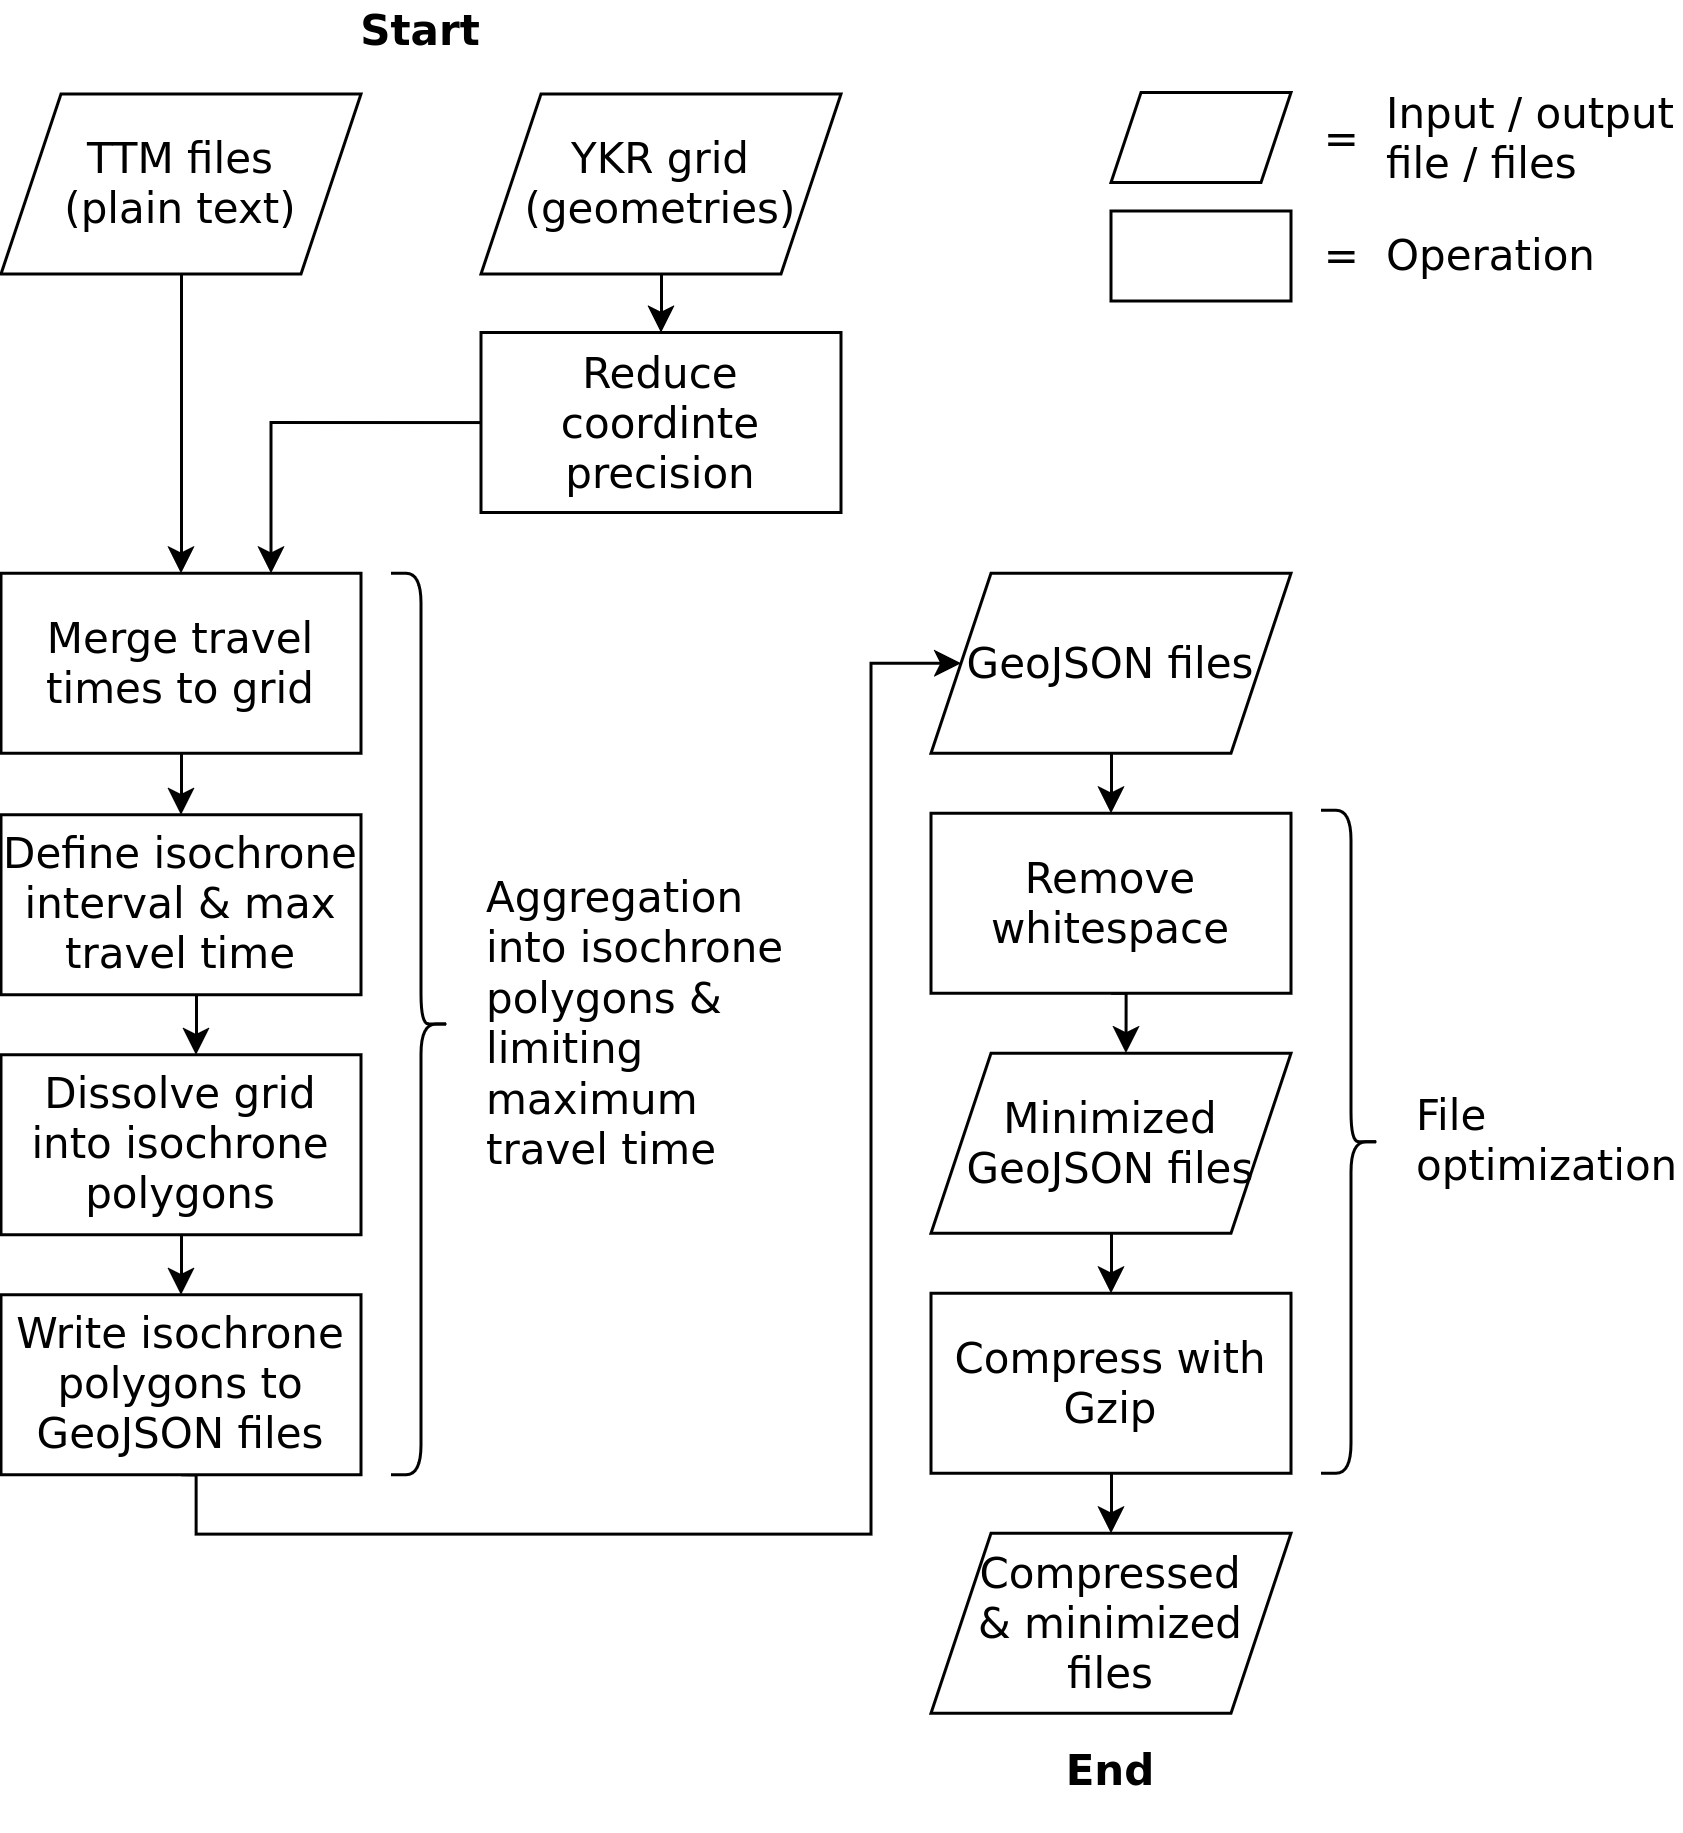
\includegraphics[width=0.8\textwidth]{visual/figures/diagrams/preprocessing.png}
	\caption{Preprocessing}
	\label{fig:preprocessing}
\end{figure}


\subsubsection{Constructing the map application}

The need for visualization (frontend) and the requirements visualization must satisfy

Different approaches

Why react? Why not just make a map?
The map is a map, but it is also a user interface that controls state outside the map.
Integration with react means more robust code, better developer experience and maintainability.
Do not reinvent the wheel.

% TODO Describe why these libraries were selected
Basis for the map library comparison

Baseline: FOSS, Actively maintained, usable with UI framework (react)

Initial contenders: Leaflet, Openlayers, Mapbox, Maplibre, Deckgl

Instantly discarded: Openlayers (non-existent integration to react) Mapbox (non-foss)

% TODO copypasta
Translucent Overlay (OV) is the best technique over-
all, which makes it a good choice when only one comparison
technique should be provided to user \parencite{lob2015}.

% Describe how it was done



% I see the methods necessary to implement the visualisation belonging to two themes:
% Methods for figuring out how the map should be
% and methods for actually making the map be that way.

% For figuring out what the map should be like,
% I have (hopefully) at this point already formed some ideas from the background section.
% To complement those, and to keep the qualitative aspect of cartography relevant,
% interview(s) will be used alongside the development process.

% When developing the visualisation, the priority should be on the map application.
% However, the development must progress on all components as an iterative process,
% where producing a minimal working state should be the first goal.
% Something that, to some extent, works, makes discussion about the map possible,
% which in turn should keep development progressing towards the right direction.

% It should also be noted that the number of techical options for implementing the map is large.
% Questions such as which mapping library or UI framework to use,
% or how to preprocess the matrix data should be covered here too.
% Depending on the need and extent of comparisons between different technologies,
% some synthesis could be formed about that too.

\subsubsection{Technical architecture}

\begin{figure}[H]
	\centering
	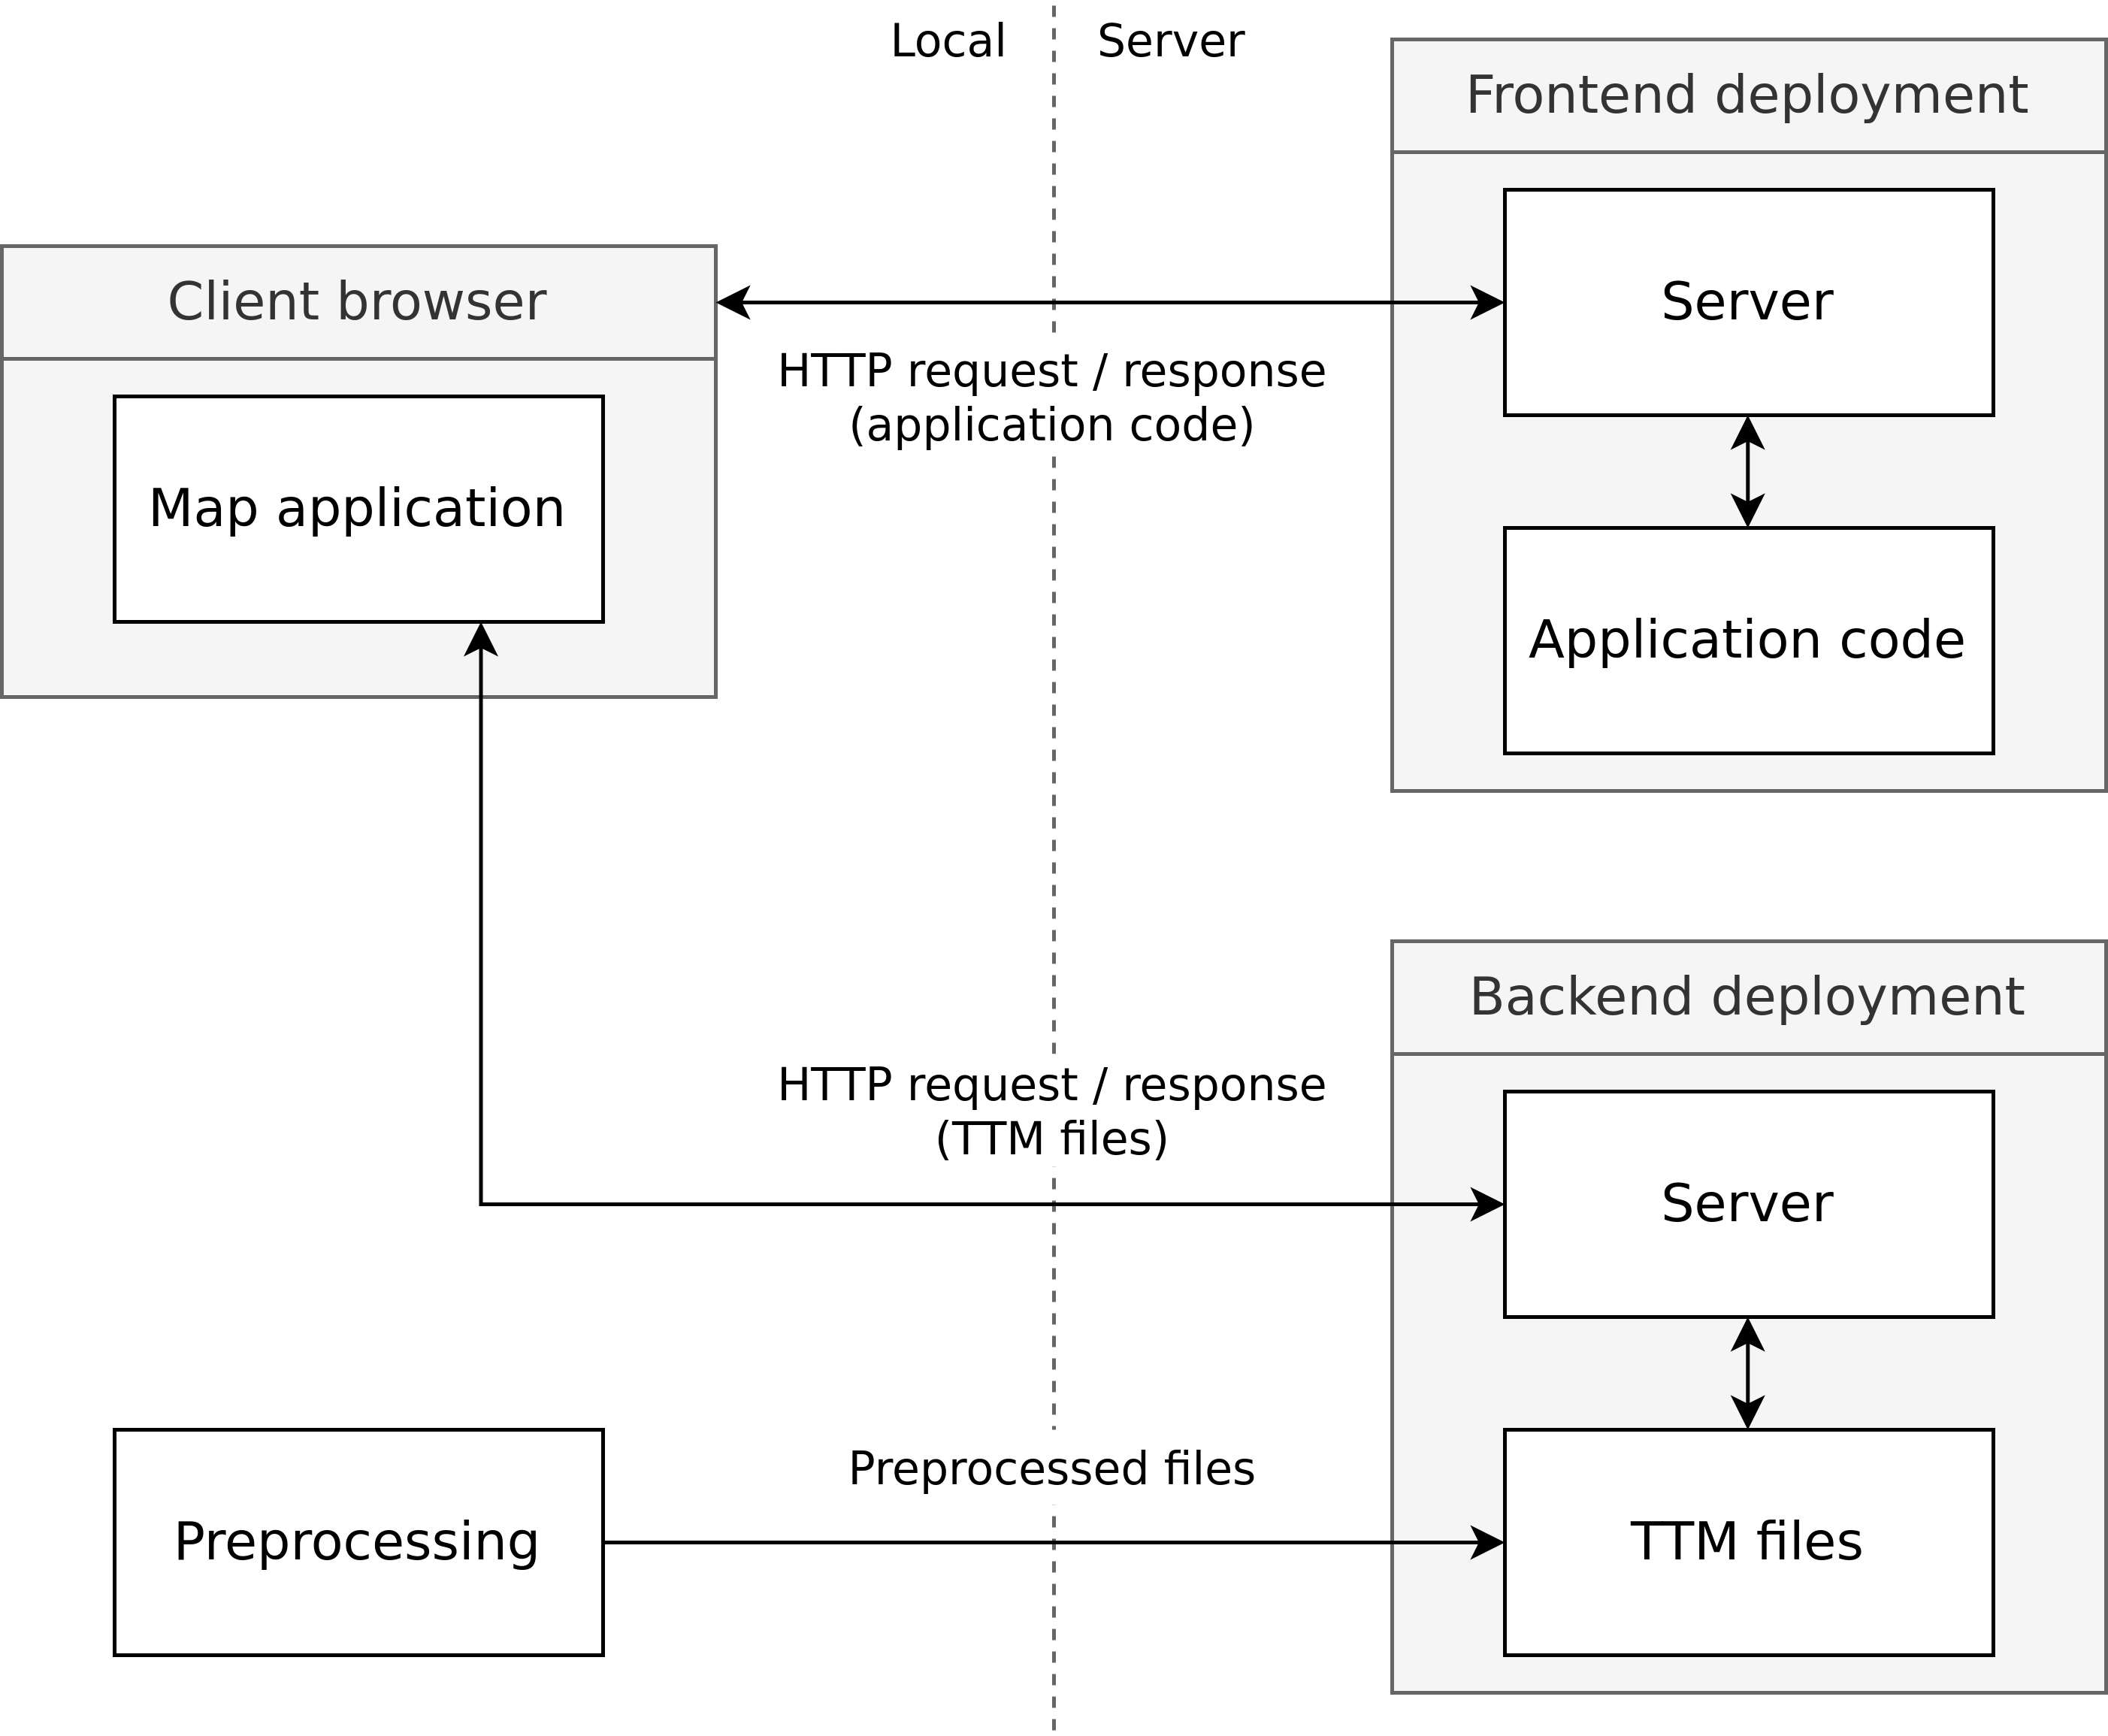
\includegraphics[width=0.8\textwidth]{visual/figures/diagrams/architechture.png}
	\caption{Architecture}
	\label{fig:architechture}
\end{figure}


% The need for serving (backend)
% - why data must be decoupled
% && the requirements serving must satisfy

% Different approaches

% Why nginx + static files?

% Describe how it was done

\subsection{Survey}
General reasoning about the survey

\subsubsection{Questionnaire design and structure}
The content of the questionnaire: prompts and questions

\subsubsection{Survey process}
The content of the questionnaire: prompts and questions

\subsubsection{Participants}
Descrtiption of the collected data
